
    
\begin{comment}
\chapter{Data Colection} % Main chapter title

\label{Chapter3}
Before deciding the best approach to the problem, a thorough analysis of the data was needed. Firstly the model of the robotic arm had to be analized, then a virtual simulation of the robot was created in CoppeliaSim. The data was then collected from the simulation and analyzed.\\

\section{Collaborative robot UR5}

The Universal Robots UR5 stands out within the collaborative robotics arena, exemplifying the integration of advanced robotic technology and human-centric operational capabilities. This section delves into the UR5 robotic arm's key characteristics, its operational paradigm, and the underlying mathematical model that enables its precise movements and interactions within collaborative settings.\\
Originating from Universal Robots, a Danish innovator in the field of robotics, the UR5 robot is part of the UR series, which also includes the smaller UR3 and the larger UR10 models. 
The series is distinguished by its payload capacity, denoted by the numerical value in each model's name, indicating 3 kg, 5 kg, and 10 kg for the UR3, UR5, and UR10, respectively. 
Designed for versatility and ease of use, the UR5 embodies the essence of collaborative robotics, offering a harmonious blend of advanced technology and user-friendly interfaces.\\
The UR5 robotic arm is celebrated for its:


\begin{itemize}
    \item \textbf{Ease of Programming:} The robot's programming interface, facilitated by a touch screen known as the teach pendant, is designed for intuitive use, significantly reducing the learning curve for operators.
    \item \textbf{Operational Flexibility:} Marked by its lightweight design and compact form factor, the UR5 can be easily repositioned and redeployed for a wide range of tasks, enhancing operational agility.
    \item \textbf{Direct Human-Robot Collaboration:} With safety at its core, the UR5 is engineered to work alongside human operators, seamlessly integrating into shared workspaces without the need for physical barriers.
    \item \textbf{Peripheral Compatibility:} The robot supports a vast array of external devices and tools, enabling customization and versatility across various applications.
    \item \textbf{Consistent Quality Output:} The precision and reliability of the UR5 make it an ideal solution for tasks requiring high levels of accuracy, such as assembly and material handling.
\end{itemize}

The UR5 system comprises three main components:

\subsectionautorefname{Control Unit}
The control unit, houses the CPU, safety management module, and USB hub. 
It orchestrates the robot's movements, ensuring smooth and safe operations. Key functionalities include:
\begin{itemize}
    \item \textbf{CPU:} Serves as the primary processing unit for the robot, executing instructions from the operating system and application software. 
    It performs calculations, processes data, and controls the logic operations essential for robot functionality. 
    The CPU enables the robot to interpret and execute commands, manage its sensors and actuators, and maintain connectivity with external devices or networks for control and data exchange.
    
    \item \textbf{Safety Management:} Comprises hardware and software mechanisms designed to monitor and control the robot's operations to prevent accidents and ensure the safety of human operators and other machinery in the environment. 
    This module continuously evaluates safety-related signals from the robot's sensors and executes predefined emergency protocols or safety functions in response to potential hazards. 
    Its responsibilities include enforcing operational limits, managing error detections, and implementing emergency stop functionalities.
    
    \item \textbf{Software Housing:} Refers to the storage medium within the control unit that contains the robot's operating system (OS), user interface (UI) software, and the programming framework that supports robot application development and execution. 
    The operating system manages the robot's hardware resources and provides services for application software. 
    The user interface allows for interaction between the robot and its operators, facilitating programming, configuration, and monitoring of robot activities. 
    The programming framework provides libraries, tools, and APIs necessary for developing robot applications, defining task sequences, and integrating custom functionalities.

\end{itemize}


\subsection{Robotic Arm}
The robotic arm of the UR5 collaborative robot is designed with a modular architecture, offering six degrees of freedom to ensure versatile and precise maneuvering. This section outlines the technical specifications and operational capabilities of the UR5 robotic arm, emphasizing its engineering design, functional components, and integration within the collaborative robotics framework.
The UR5 arm is constructed with lightweight materials, allowing for a payload capacity of up to 5 kg. Its mechanical structure comprises six revolute joints, each powered by a servo motor. These joints enable the arm to perform complex tasks by extending, retracting, lifting, and rotating objects within its operational range.

\begin{itemize}
    \item \textbf{Degrees of Freedom:} Six revolute joints facilitate a wide range of motion, allowing the arm to approach tasks from virtually any angle.
    \item \textbf{Reach and Workspace:} The arm has a maximum reach of 850 mm, providing an expansive workspace to perform tasks efficiently.
    \item \textbf{Payload Capacity:} Designed to handle loads up to 5 kg, catering to a variety of applications from material handling to precise assembly tasks.
    \item \textbf{Speed and Precision:} High-speed servo motors ensure rapid and accurate positioning of the arm, enhancing productivity and operational efficiency.
\end{itemize}
The UR5 arm integrates several key components to achieve its high level of functionality and reliability:

\begin{itemize}
    \item \textbf{Servo Motors:} Each joint is equipped with a high-torque servo motor, enabling precise control over the arm's movement and position.
    \item \textbf{Encoders:} High-resolution encoders attached to each joint provide real-time feedback on the arm's positional data, facilitating accurate motion control.
    \item \textbf{End-Effector Interface:} A versatile end-effector interface allows for easy attachment and detachment of various tools and grippers, expanding the robot's application range.
    \item \textbf{Safety Sensors:} Integrated safety sensors ensure collaborative operation with human operators, automatically stopping the arm if a potential collision is detected.
\end{itemize}



\subsection{Mathematical Model and Kinematics}
Understanding the UR5 robot's motion within its operational space necessitates an exploration of its mathematical model, with direct kinematics being central to this investigation. 
This model enables the conversion of joint angles to the precise position and orientation (pose) of the end effector.
Key aspects include:

\begin{itemize}
    \item \textbf{Direct Kinematics:} The UR5 robot can be conceptualized as a kinematic chain of rigid bodies (links), interconnected through either revolute or prismatic joints. 
    This chain extends from a fixed base to a mobile end-effector. The goal of direct kinematics is to determine the pose of the end-effector given the configuration of the robot's joints.
    \item \textbf{Denavit-Hartenberg Convention:} The Denavit-Hartenberg (D-H) convention offers a systematic way to describe the geometry of the robot arm, facilitating the mathematical modeling of direct kinematics.
    It assigns four parameters to each link in the kinematic chain: the link length ($a_i$), link twist ($\alpha_i$), link offset ($d_i$), and joint angle ($\theta_i$). 
    These parameters, known collectively as D-H parameters, define the spatial relationship between consecutive links.\\
    Given the D-H parameters, the transformation from one link to the next is represented by a $4 \times 4$ homogeneous transformation matrix. 
    This matrix incorporates rotations and translations that relate the coordinate frames attached to adjacent links.
    
    \item \textbf{Inverse Kinematics:} Inverse kinematics addresses the calculation of joint configurations necessary to achieve a specific end-effector pose. 
    Unlike direct kinematics, it involves determining the joint parameters that result in the desired position and orientation of the robot's end-effector.

    \item \textbf{Control Law and Jacobian Inverse:} To perform precise movements, the UR5 employs a control strategy based on inverse kinematics, using the Jacobian matrix to relate joint velocities to end-effector velocities. 
    The Jacobian inverse is pivotal for converting desired end-effector velocities into joint velocities, allowing for dynamic adjustments to the robot's posture and ensuring the execution of complex tasks.
    The Jacobian matrix ($J$) is crucial for understanding the relationship between joint velocities ($\dot{q}$) and end-effector velocities ($\dot{x}$). 
    It is derived from the geometric Jacobians associated with each joint, compiled into a comprehensive matrix that models the robot's kinematics.

\end{itemize}
     
The UR5's kinematics model was then loadoded into the CoppeliaSim simulator, to create a virtual model of the robot.


%SECODN SECTION --------------------------------------------------------------------------------------------------------------------------------------------------------------------------
\section{Coppeliasim}

CoppeliaSim, previously known as V-REP (Virtual Robot Experimentation Platform), is recognized for its versatility and scalability as a robot simulation framework \cite{coppeliasim2023}  and \cite{ur5manual}. 
It enables the rapid and accurate simulation of complex physical scenarios leveraging a robust physics engine. 
In a simulation scene, various objects such as shapes and vision sensors are organized hierarchically in a tree structure.
CoppeliaSim's design embodies a flexible architecture that supports multiple programming approaches, thus providing versatility in the execution of control code. 
    
\begin{figure}[H]
        \centering
        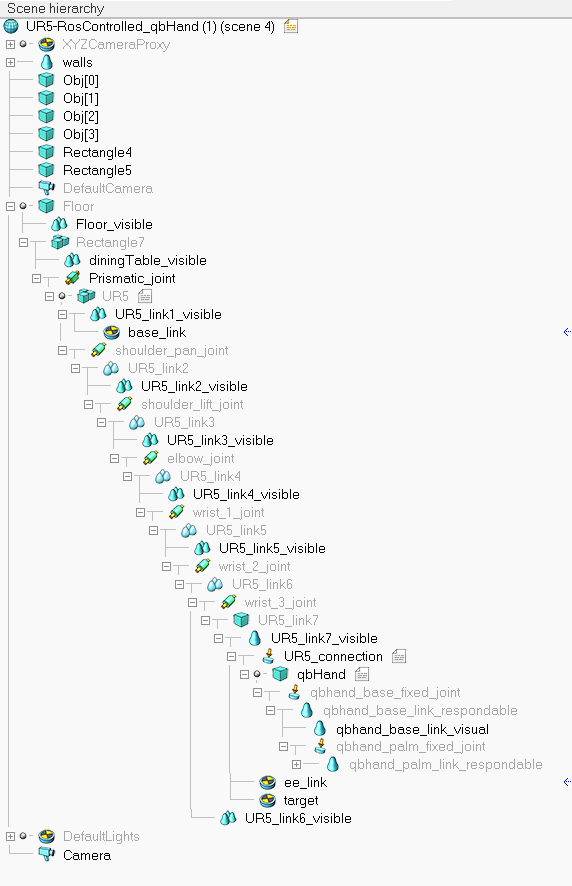
\includegraphics[width=0.4\textwidth]{Figures/Chapter3/sceneHierarchy.png}
        \caption{Roboto arm Model Hierarchy}
        \label{fig:RobotArmHierarchy}
\end{figure}

The integration highlights the following programming paradigms:
\begin{itemize}
    \item \textbf{Embedded scripts:} Written in Lua, these scripts are associated with scene objects as child scripts. A main Lua script, acting as the simulation loop, oversees general functionality and orchestrates the execution of child scripts based on the scene hierarchy. 
    These child scripts are tied to specific objects, managing particular elements of the simulation. This structure of modular and distributed embedded scripts enhances their effectiveness.
    \item \textbf{Remote application programming interface (API) clients:} CoppeliaSim's remote API facilitates interaction with the simulation environment via socket communication. 
    It supports server services and client applications in various programming languages, including C/C++, Python, Java, MATLAB, and Urbi, enabling remote function calls and fast data streaming.
    \item \textbf{Add-ons:} Operated through Lua scripts, add-ons can act as either standalone utilities or code executed at regular intervals, expanding the simulation's capabilities.
    \item \textbf{Plug-ins:} These are utilized for simulator customization, allowing for the registration of custom Lua commands and the extension of functionality within simulation models or objects.
\end{itemize}

CoppeliaSim allowes integration with ROS, allowing to control the robot from the ROS environment.\\
The initial step in the integration process involves establishing a communication link between CoppeliaSim and ROS. 
This is typically achieved through the use of a dedicated ROS package, such as \texttt{coppeliasim\_ros\_interface}, which facilitates direct interaction between CoppeliaSim's simulation environment and ROS nodes. 
The package utilizes CoppeliaSim's remote API capabilities to create a bridge that allows for the bidirectional exchange of information and commands.\\
Once the connection is established, ROS can control simulated robots within CoppeliaSim by publishing messages to specific topics that correspond to the robots' actuators and sensors. 
This setup enables the simulation of sensor data acquisition, actuator control, and even complex robotic behaviors such as navigation, manipulation, and interaction with dynamic environments.\\
ROS nodes can subscribe to CoppeliaSim's simulated sensors' data, such as camera feeds, laser scans, or joint states, allowing for real-time monitoring and decision-making. 
Similarly, nodes can publish commands to control the simulated robot's movements, manipulator positions, or any other actuator-driven actions, mimicking the control flow of a real robot.\\

The joint limits were configured to match the real robot. 
\begin{table}[h!]
    \centering
    \begin{tabular}{| m{2cm} | m{4cm} |}
    \hline
    \textbf{Joint Number} & \textbf{Joint Limitation} \\
    \hline
    1 & +/- 360° range \\
    \hline
    2 & +/- 360° range \\
    \hline
    3 & +/- 360° range \\
    \hline
    4 & +/- 360° range \\
    \hline
    5 & +/- 360° range \\
    \hline
    6 & +/- 360° range \\
    \hline
    \end{tabular}
    \caption{Joint limitations of the UR5 robot}
\end{table}


%THIRD SECTION --------------------------------------------------------------------------------------------------------------------------------------------------------------------------
\section{Data Collection}


\end{comment}



  